% This is samplepaper.tex, a sample chapter demonstrating the
% LLNCS macro package for Springer Computer Science proceedings;
% Version 2.21 of 2022/01/12
%
\documentclass[runningheads]{llncs}
%
\usepackage[T1]{fontenc}
% T1 fonts will be used to generate the final print and online PDFs,
% so please use T1 fonts in your manuscript whenever possible.
% Other font encondings may result in incorrect characters.
%
\usepackage{graphicx}
% Used for displaying a sample figure. If possible, figure files should
% be included in EPS format.
%
% If you use the hyperref package, please uncomment the following two lines
% to display URLs in blue roman font according to Springer's eBook style:
%\usepackage{color}
%\renewcommand\UrlFont{\color{blue}\rmfamily}
%\urlstyle{rm}
%
\usepackage{amsmath,amsfonts}
\usepackage{algorithmic}
\usepackage{algorithm}
\usepackage{array}
\usepackage[caption=false,font=normalsize,labelfont=sf,textfont=sf]{subfig}
\usepackage{textcomp}
\usepackage{stfloats}
\usepackage{url}
\usepackage{verbatim}


%% biblatex
\usepackage[style = numeric, backend = biber, sorting = none, doi = false, isbn = false, url = true]{biblatex}
% \usepackage[defernumbers = true, style = numeric, backend = biber, sorting = none, doi = false, isbn = false, url = true]{biblatex}
% \usepackage[style = numeric, backend = biber, sorting = none]{biblatex}    % REFERENCIAS como section
\AtEveryBibitem{
    \clearfield{urlyear}
    \clearfield{urlmonth}
} % Do not show the "(visited on <date>)" on the references
\DefineBibliographyStrings{spanish}{}
\usepackage{csquotes}
\addbibresource{./bettachini.bib}
\renewcommand*{\bibfont}{\fontsize{9}{12}\selectfont}

\usepackage{xcolor}
\newcommand{\MR}[1]{{\color{magenta}#1}}

\usepackage[normalem]{ulem}




\begin{document}
\title{A code-centric flipped classroom course on analytical mechanics}

%\titlerunning{Experiences on a Comp. Anal. Mech. course...}
% If the paper title is too long for the running head, you can set
% an abbreviated paper title here


%
\author{
	Víctor~A.~Bettachini\inst{1,2}\orcidID{0000-0001-7485-8884} \and
	Mariano~A.~Real\inst{1,3}\orcidID{0000-0003-3022-7516} \and
	Edgardo~Palazzo\inst{4}\orcidID{0009-0006-8783-8261}
}
%
\authorrunning{V. A. Bettachini et al.}
% First names are abbreviated in the running head.
% If there are more than two authors, 'et al.' is used.
%
\institute{
Universidad Nacional de La Matanza - UNLAM, Buenos Aires, Argentina 
\email{vbettachini@unlam.edu.ar}\\
\url{https://ingenieria.unlam.edu.ar/} 
\and
Instituto Geográfico Nacional - IGN, Buenos Aires, Argentina
\and
Instituto Nacional de Tecnología Industrial - INTI, Buenos Aires, Argentina
\and
Universidad Tecnológica Nacional - UTN, Buenos Aires, Argentina\\
}


%
\maketitle              % typeset the header of the contribution
%
\begin{abstract}
%The abstract should briefly summarize the contents of the paper in 150--250 words.
This paper outlines the methodologies, tools and organisation of mechanical engineering undergraduate course that employs code as the sole means to perform all its calculations. Modeling simple mechanical devices as rigid bodies and employing the analytical mechanics Euler-Lagrange equation the code is able to simulate the dynamics and mechanical efforts of these systems. No prior programming skills are required, provided code that solves example problems is modified by students to address new ones. Jupyter Notebooks running on Google Colaboratory provides an unified platform for lesson's material embedding code among Markdown formatted text and \LaTeX\ mathematical expressions. 

Originally conducted online during the SARS-CoV-2 pandemic, the course has transitioned to in-person sessions and a flipped classroom approach. Exercises sets turn-in is mandatory but keeping overall homework at the minimum to free-up student's time for reading of lessons before weekly face-to-face meetings that provide opportunities for clarification and progress discussions. A learning management system is used to keep track of each student progress and to provide asynchronical consultations.

The course culminates in a challenging final problem: analysing forces and torques on a simplified industrial robotic arm. Beyond technical skills, students enhance presentation and synthesis abilities, defending their solutions through concise oral presentations to teachers.


\keywords{Code \and Flipped Classroom \and Mechanical Engineering}
\end{abstract}

%
%
% \section{Summary}
% “Numerical Analysis” and “Programming Fundamentals'' are mentioned as “Knowledge Descriptors'' for a Mechanical Engineer in the “Proposal of standards for the second generation for engineering degrees accreditation in the Argentine Republic” 
%(“Propuesta de Estándares de Segunda Generación para la Acreditación de Carreras de Ingeniería en la República Argentina”) 
approved by the “Federal council of engineering deans” %(Consejo Federal de Decanos de Ingeniería, CONFEDI) 
in 2018, and best known as “Libro Rojo de CONFEDI”\cite{librorojo}. 
Regrettably after theory and use of these tools are learnt by students they are not fully exploited in courses at later years.

In this work the experience had at the subject Mecánica General (General Mechanics) of the UNLaM’s mechanical engineering degree third-year is described. Traditionally modeled systems are limited to those analytically solvable working on blackboard or paper. In this course the students solve their problem sets using Python language code, applying this century tools, such as library functions for symbolic and numerical analysis, plotting, etc.

All classes were conducted in full using Jupyter notebooks as a platform. In those notebooks code  is interbowen with graphical information and text including clear mathematical notation with LaTeX symbols. Students can re-use this same code to solve course’s problem sets as well as in future courses and their professional life.

The notebooks mentioned above run  on free software. Students operate on them with free to use web platforms that  allow concurrent commenting and editing among them and/or their professor.

The pandemic pushed us all to teach through a computer. After an initial adaptation period the students recognized the virtues of this methodology. Even assessments were more enriching than in a conventional course as it reached the complexity of simulating industrial-like mechanical systems.


% “Fundamentos de programación” y “Cálculo numérico” se mencionan entre los “descriptores de conocimiento” para un Ingeniero Mecánico en la “Propuesta de Estándares de Segunda Generación para la Acreditación de Carreras de Ingeniería en la República Argentina” aprobado por el Consejo Federal de Decanos de Ingeniería (CONFEDI) en 2018, mejor conocido como “Libro Rojo de CONFEDI”. Lamentablemente tras que la teoría y uso de estas herramientas son aprendidos por los alumnos no suelen aprovecharse en profundidad en cursos de años posteriores.

% En este trabajo se describe la experiencia que se tuvo en la asignatura Mecánica General del 3.er año de la carrera en la UNLaM. Tradicionalmente los sistemas modelados se limitan a los resolubles analíticamente por trabajar en pizarrón o papel. En este curso, los estudiantes resolvieron sus ejercicios utilizando código en lenguaje Python, haciendo uso de herramientas de este siglo, como bibliotecas de funciones para el cálculo simbólico, numérico, graficación, etc.

% Todas las clases se dictaron íntegramente usando cuadernos de Jupyter como plataforma. En estos se intercala código con información gráfica y texto incluyendo una clara notación matemática con simbología LaTeX. Este código es re-utilizable por el estudiante para resolver la ejercitación del curso con la misma herramienta, así como para ser aprovechado en asignaturas futuras y en su vida profesional.

% Estos cuadernos se ejecutan sobre software libre. Plataformas web de acceso gratuito a través del navegador permitieron a los estudiantes ejecutarlos en su hogar o trabajo, permitiendo comentar y editar en forma conjunta un mismo cuaderno entre alumnos y/o docentes.

% La pandemia nos forzó a enseñar a través de una computadora. Tras un periodo inicial de adaptación los estudiantes reconocieron las virtudes de esta metodología. Inclusive la evaluación fue más enriquecedora que en un curso convencional al alcanzar la complejidad de simular sistemas mecánicos similares a los industriales.\par\bigskip


\section{Introduction}

\subsection{Valuing teachers' and students' time}
The psychologist J.C.R. Licklider stated in the 1950s that 85\% of his ``thinking'' time was in fact used in information related tasks such as finding it or plotting graphs; an observation that set him to become an advocate of interactive computing and push the creation of ARPANET the antecessor to today's INTERNET \cite{waldrop_dream_2001}.
In the 21st century, it is not unusual to find university courses following a routine where professors transcribe lessons by heart to blackboards or repeat slide presentations. Students then transcribe this information once again into their paper or digital notebooks, a methodology largely unaltered since its introduction in the 19th century.
The situation is aggravated in science and engineering courses, where the same calculations and drawings are made repeatedly, not only in the classroom but also when exercises based on the subject of the class require performing very similar tasks to those done by the teachers.

This excercise on repeated transcription can be seen as a waste time due to the ubiquitous availability of technologies product of the information revolution during the last half of the 20th century propelled by the efforts of Licklider and colleagues.
Trying to avoid this our university course harness the power of interactive computing for in-class lessons as well as for solving problem sets using the same digital platform. 
All material that the teaching staff want to share to students is in a digital format that not only contains all theory on the subject but code that solves problems related to it.
A document containing executable code for each lesson is stored in a public repository from where the students generate their own copy.
The copy's code is fully modifiable, and students are required to do so in order to solve the problem sets proposed by the teaching staff in a procedure akin to recycling.
The matematician S. Papert, a pioneer of employing computers in a constructivist framework for education, onec stated that learning takes place when the learner takes charge of the operation \cite{papert_childrens_1993}.
Following this advise, the problem-sets in our course are built to lead the student gradually to becoming autonomous by reusing not the code provided by the teaching staff but his own code to address increasingly more complex problems.

In the current century, the fact that university courses do not ubiquitously employ coding to save time an effort of everyone in our classrooms is a situation alike the rejection of pocket calculators in 1970s argumenting that abilities on arithmetics would be jeopardised \cite{roberts_impact_1980}.
Nowadays after students learnt arithmetics at elementary school they can freely use pocket calculators.
The same should be the case after they passed their calculus and algebra courses, they should be able to employ freely their computational counterparts in all their following courses.
Not only would the focus of their effort be diverted from those automatable calculations, but they could also tackle with the tools of numerical analysis problems beyond what can be solved on a blackboard or on paper.


\subsection{Numerical analysis and computers}
The stored-program digital computer was conceived as a more flexible tool for solving numerical analysis problems than their electro-mechanical predecessors that had to be reconfigured to address different problems \cite{kurrer_konrad_2010}.
Originally funded by and reserved for military research programs at the forties, it was towards the end of that decade that civilians at universities started to exploit them for other purposes \cite{simon_h_lavington_history_1975}. 
So, PhD candidates were among the first students to use these mainframe computers in the so called punch card and batch processing era that stretched into the 1970s. 
By then, higher-level languages and lower-cost minicomputers had opened up access for undergraduate students \cite{kemeny_dartmouth_1968}.
Time-sharing based live interaction with computers became an established practise, allowing to serve several students at once to deploy computer-based instruction \cite{tidball_using_1978}.
These computer-assisted instruction systems provided tailor-made lessons created by the teaching staff, alongside questionnaires and other interactive feedback mechanisms to evaluate students' understanding of a variety of subjects. This approach avoided pressuring students into programming \cite{cope_little_2023}.
A contemporary push on the opposite direction directed to school age students sought to foster mathematical and geometrical abilities, creating languages aimed for educational use based on ideas of the constructivist philosophy \cite{ben-ari_constructivism_1998}, such as LOGO \cite{solomon_history_2020} or Smalltalk \cite{kay_early_1993}.

Coming full circle to the origin of digital computers, exploitation of numerical analysis by undergraduate students performed with languages such as Python, that inherits the simplicity of LOGO and object orientation of Smalltalk, could provide them a useful calculation tool at almost any science or engineering course.
As digital pocket calculators freed students of repetitive arithmetic tasks, allowing to explore otherwise avoided problems, current programming languages provide symbolic and numerical analysis as well as plotting capabilities that allow to visualise and explore the mathematical solutions of any conceivable problem presented in university courses.


\section{Course cornerstones: code reuse and flipped classroom}

\subsection{Analytical mechanics for mechanical engineers}
Numerical analysis courses are ubiquitous in the mechanical engineering degrees programme's firsts years in the Argentine Republic.
There are usually preceded by a course on programming fundamentals, allowing to focus the efforts of the teaching staff of the former to rely on what was taught in the later.
Unfortunately it is not unusual that in later courses the problems presented to students are limited to those 
having analytical solutions of the models, so the knowledge and practice obtained not only on the subject of numerical analysis, but also of programming as a tool, are seldom exploited at full at later courses.
In an effort to revert this trend, our course on analytical mechanics precedes those later ones and is placed immediately after those where these abilities were acquired. 
As shown by the roadmap presented in Figure \ref{fig:correlativas} for the degree on mechanical engineering at La Matanza University (UNLaM).
One reason to do so, is to put mechanical engineering students to work on the subject matter of mechanical devices quickly, capitalising what they learnt in subjects devoted to algebra, mathematical analysis, numerical calculus, and Newtonian mechanics.
Another reason is to assure the teaching staff of the subjects on the mechanics of stability, devices or fluids, that the students they receive are experienced on the tools of analytical mechanics but also on computer-based numerical analysis.
In this way the course acts as a link between the first specific mechanical courses and the basic ones.

\begin{figure}[ht]
\centering
\includegraphics[width=0.9\linewidth]{figuras/ubicacion}
\caption{Preceded by subjects of algebra, calculus, and physics, analytical mechanics is the first in which such knowledge is applied to mechanical engineering.
It also serves as a foundation for subsequent specialised mechanical engineering courses.}
\label{fig:correlativas}
\end{figure}

But, why is the physics subject of analytical mechanics, also known as classical mechanics, a worthwhile tool for mechanical engineers? 
The mere statement that it confers the power to model the physics of simple mechanical systems does make it sound like a redux of Newtonian mechanics.
And it is in putting in contraposition with that another philosophy of how to understand physical mechanics that the value of the analytical approach stands appart.
Instead of an artisanal analysis of vector forces, the analytical approach is absolutely systematic.
Creativity is only required to produce a physical model out of the observation of the actual system, then it follows the same identical steps, independently of the system under study, to produce results, making it highly automatable for machines or people alike \cite{cornelius_lanczos_variational_1952}.
The creation of a physical model from observations involves simplifications, the student must determine what is important and what is not to capture the main features of the physical system.

Training this ability of students is the most demanding challenge  to the teaching staff of this course.
Once a physical model is constructed the analytical mechanics steps based on the Euler-Lagrange formalism, reviewed later in this work, produce a set of differential equations.
These can describe the dynamics or the mechanical efforts the actual system is subjected to, and next one needs only to solve them.


\subsection{Limits on analytical mechanics usefulness}
Traditionally, the physical systems studied in analytical mechanics courses are relatively simple in order to limit the time and/or difficulty of mathematical analysis and/or algebra calculations required by the steps commented in the previous paragraph.
But this extreme simplification leads to a later noticeable jump in the complexity required to model mechanical devices, fluid dynamics, or rigid structures, in the courses, shown in the figure \ref{fig:correlativas}, coming up next where the student must apply this tool.
The limitation to complexity of the examples is imposed by what can be calculated on a blackboard or presentation slides.
The same goes for the length and complexity of the problems that students can be asked to solve.

Computer algebra systems, that will soon turn 60 \cite{ams}, have of course certain limitations on what they can compute, but these are well beyond of the most complex problem an undergraduate student of engineering could meddle in.
Libraries for symbolic algebra and calculus are available for all major general programming languages, both libraries and languages being published as free software.
So the only reason that limits the reach of what students can calculate is a culture that keeps the blackboard, slides or paper as the centre piece of the work at classrooms in place of computers.
Although numerical analysis is reportedly used to solve problem sets \cite{mirasso-raichman, caligaris-rodriguez}, it is rarely used by the teaching staff during classes.
But if the application of numerical analysis during classes is rare, the use of symbolic computer algebra is even rarer.
The use of computer algebra and calculus solutions re-focus the students attention towards the subject matter of the current course.


\subsection{Programming vs. code reuse}
Having fluency in a computer language's code in order to be able to comprehend what was written by another person, modify it or even write its own is of course an ability required for programming, but by itself fells short of the analytical skills and knowledge of algorithms and computer architecture required by professionals in the field.
For the matters of our course we state a strict distinticion between ``programming'' and the less demanding ``coding'' to the students at the first meeting they have with the teaching staff.
Altough at UNLaM they had a previous course of introduction to programming based on \verb!C++!, so they already posess ability on programming algorithms, that in any way is something they need to apply in the course.
In our experience, even for students that allegedly ``have forgotten'' what they learnt on programming due to lack of use found that Python's concise and simple syntax \cite{perkel_programming_2015} makes it relatively accesible to grasp it to the level required to understand and modify the code provided by the teaching staff.

For each class the teaching staff makes available examples of codes that perform all the procedures required to model a certain characteristic of a mechanical system.
Related exercises are provided in a problem set that can be solved by making small modifications to the code.
This later ability to adapt the code by slight changes is nothing more than code reuse, a common practice in the computing industry since its inception.

A good deal of courses appeared during the last decade that take advantage of tools such as the ones used in our course, to produce graphical output to clarify the results of numerical simulations in diverse areas such as computational fluid dynamics \cite{barba_cfd_2018} or chemical thermodynamics \cite{vallejo_google_2022}.
There are also teaching materials, once again relying on these tools, that are published in a book alike format in the fields of chemistry \cite{weiss_creative_2021}.
But these cited examples used their published material containing code to support the lessons, not to be the basis of their problems sets.
There are of course others that do exactly that, even providing example problems with the code required to solve them embedded into them, such one on stucture modelling for civil engineers \cite{laureline_duvillard_using_nodate}, but these do not rely on the media to be the basis for their lessons.
We understand that not using the same digital format with embedded code both at lessons and to solve the problem sets results in the exercise of transcription discussed previously. 
To the best of our knowledge there is no course, besides ours, that integrates analytical mechanics with numerical analysis in lessons to provide code able to calculate problems of dynamics and efforts in rigid body mechanical systems using the same digital media.


\subsection{Flipped classroom}
The course first edition was coincidental with the outbreak of the SARS-CoV-2 pandemic.
Lockdowns forced us to implement emergency remote lessons based on digital teleconference software solutions.
The teaching staff having previously used Jupyter Notebooks at laboratory courses wrote the lessons for the first weeks taking advantage of Python code to perform the required calculations and also plotting its results.
While the first synchronical meeting was conducted, it was verified that each one of the students was sitted in front of a computer.
The opportunity to force students to use code to solve the exercises set was quickly grasped.
After an initial adaptation period, the students recognized the virtues of this methodology. 
Even assessments were more enriching than in a conventional course as it reached the complexity of simulating industrial-like mechanical systems.
During the four semesters when lessons were remote, adoption of asynchronous consultations grew.
As the lesson material was published in advance to the meetings, the teaching staff started to suggest that it be read before it in order to discuss it rather than present it.
This then led to suggest that some excercises be solved also in advance.
Gradually this led to free time at the meetings thus allowing the students to work on the excercises while they could make synchronical consultations on them to the staff.
By the time in person meetings at classrooms began, the staff decided to put to test a radical proposal: avoid giving lectures altogheter, switching to the \textit{flipped classroom} methodology \cite{oflaherty_use_2015, noauthor_flipped_2024} schematised in figure \ref{fig:flippedClassroomSchedule}.

\begin{figure}[ht]
\centering
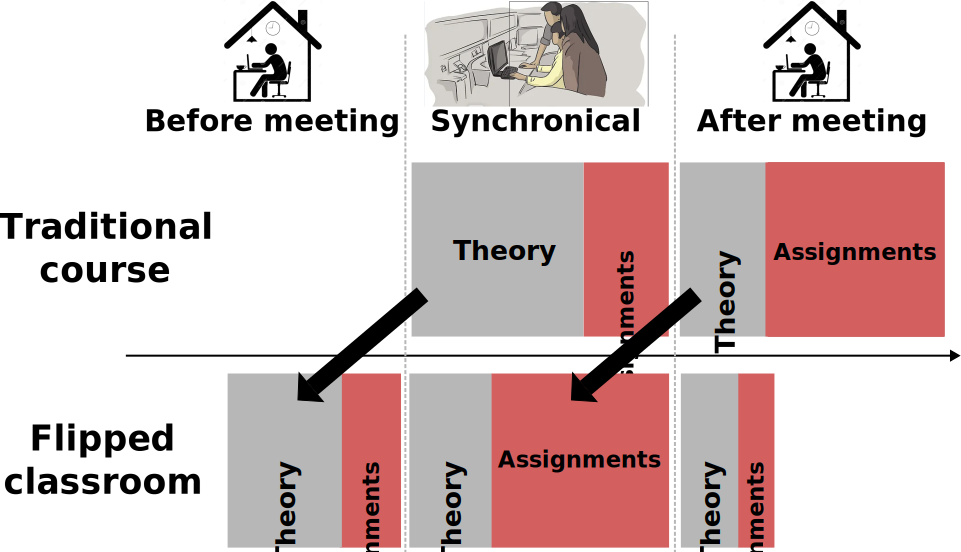
\includegraphics[width=0.9\linewidth]{figuras/flippedClassroomSchedule.pdf}
\caption{This schematizes how the student allocates the same amount of time in our flipped classroom course compared to a traditional one. There is a synchronic meeting for each thematic block. Reading theory and starting the work on their exercise set is mandatory before the meeting.}
\label{fig:flippedClassroomSchedule}
\end{figure}

The current course syllabus is strictly divided into weekly distinct thematic blocks with a single synchronic meeting devoted to it.
No lecturing occurs during the meeting, thus all the staff's available time is reserved for one to one consultations on the excercise sets.
If a single subject is perceived to need some review, a quick lecture on the particular is improvised based on the material at the repository.
Students are required to read in anticipation the respective material on theory published beforehand in the course repository as Jupyter Notebooks, alongside videos with discussions on important topics.
They also must begin working on the exercises before the meeting where they seek clarification on both, the theory and difficulties found while trying to solve the practice problems. 
As they finish up them in a later date and usually that requires some review on the theory, an asynchronic communication channel is available where the teaching staff can answer their questions on both matters.


\section{Course tools}

\subsection{Analytical mechanics and physical modeling}
The course employs the most traditional principles of rational mechanics, as outlined in standard reference literature \cite{landau}.
Modeling is understood as a series of procedures with which a simplified scheme of physics is constructed based on a semi-quantitative evaluation of the forces and fields that act on the system as well as the constraints that limit its degrees of freedom.
With such information, some of these are prioritized and others are discarded to arrive at the aforementioned scheme.
Having such a model allows:
\begin{itemize}
    \item to choose generalized coordinates to describe the relevant degrees of freedom,
    \item to write mathematical relationships between them that account for constraints,
    \item to describe generalized forces that are not the effect of fields (gravitational, electromagnetic, etc.),
    \item and to describe the potential and kinetic energy of the system as a whole.
\end{itemize}

After performing the above, the Euler-Lagrange formalism is demonstrated and put into practice in the course to obtain a set of differential equations that describe the dynamics of the system and/or the mechanical stresses that each of its components must withstand over time.

\subsection{Python, Sympy, Numpy, Scipy and Matplotlib}

The Python programming language is by default devoid of scientific and engineering calculation capabilities. 
This is a design decision to require that such functionalities be added by specialized libraries, whose development is carried out by users who apply them in various fields of science and technology.
A conscious decision was made to use the most standard and lesser in number to address the distinct requirements of the course:
\begin{itemize}
    \item Capability for symbolic algebra and calculus as provided by the Sympy library.
    Its \textit{Mechanics} module is particularly useful to generate equations for the dynamics of rigid body systems with multiple degrees of freedom and in various reference frames \cite{sympy}.
    \item Differential equation systems are solved by numerical methods supported by functions for the manipulation of algebraic elements of the Numpy library \cite{numpy} and the numerical optimization and integration algorithms of Scipy \cite{SciPy}.
    \item Engineering analysis of numerical results is usually interpreted with graphical representations. 
    This capability is provided by functions of the Matplotlib library \cite{matplotlib}.
\end{itemize}


\subsection{Jupyter Notebooks on Google Colaboratory}

The environment used in the course to run code is the web-based application called JupyterLab, whose document format is the Jupyter Notebook \cite{Kluyver2016jupyter}.
As shown by the figure \ref{fig:jupyter} these documents are divided in an arbitrary number of independent sections called cells that can contain executable code of some programming language, being Python one of the possible ones, or either annotations.

\begin{figure}[!ht]
	\centering
	\includegraphics[width=\linewidth]{figuras/screenshot_JupyterLab.png}
	\caption{
		A Jupyter notebook is a set of cells
        containing either exectuable or Markdown code.
		The former can contain text, mathematical expressions or multimedia content.
		The latter are lines of code in various programming languages.
		Interspersing titles in Markdown cells generates the index (on the left) that facilitates location within the document.
	}
	\label{fig:jupyter}
\end{figure}

Annotations cells are written in the Markdown markup language \cite{markdown} that allows to embed text and mathematical expressions in \LaTeX\ format interspersed as well as multimedia content such as web links, images, video and sound players.
The use of \LaTeX\ syntax for the mathematical symbology provides a standardised and clear notation under the guidelines of the American Mathematical Society \cite{ams}. 
This is a further advantage of the Jupyter Notebook as the media for lessons over the blackboard or slides prepared with software such as Microsoft Powerpoint.


% \subsection{Running Jupyter Online}
Students are not required to install any special software on their computer to work with Jupyter Notebooks, only a standard web browser is neeeded to use online services that run Jupyter Notebooks.
This can be an installation of JupyterHub from the Jupyter Project on university-owned servers or commercial clouds, or alternatively one of the services that offer even free alternatives such as CoCalc, IBM Watson or Google Colaboratory\footnote{The authors do no endorse any of the products or services listed here or later in this work that are mentioned only in an informative way.}.
The later, colloquialy known as Colab, is currently in use by the course as it conveniently presents the ability to run notebooks hosted by the online service GitHub.  
A modification in the URL that points to the notebook leads a web browser to open it in Colab. \cite{vallejo_google_2022,google_llc_using_2021}.
Which can be worked on concurrently by students and teachers.
Students are encouraged to collectively solve exercises using this functionality.
As shown by figure \ref{fig:colab}, comments can also be included, an useful feature to correct exercises since the location of errors in the code can be indicated.
The teaching staff can also include inline helping code and new sections into the students notebook.

\begin{figure}[!ht]
	\centering
	\includegraphics[width=\linewidth]{figuras/comentariosColab.png}
	\caption{
		The Google Colaboratoy website allows Jupyter notebooks to be edited and run concurrently between students and teachers, as well as including comments.
		The latter feature is useful for corrections.
	}
	\label{fig:colab}
\end{figure}

\subsection{Git Repository on GitHub}

The aforementioned repository on GitHub is organized into separate folders for each class of the course, as shown in figure \ref{fig:github}.

\begin{figure}[!ht]
\centering
\includegraphics[width=\linewidth]{figuras/repositorioGithub.png}
\caption{Github repository: the students find the material organized in separate directories per class \cite{repositorio-victor}.}
\label{fig:github}
\end{figure}

There is a folder for each subject matter containing the Jupyter Notebooks for lessons and exercises as well as exercise set and occasional notes in the portable document format known by its acronym in English PDF.
This arrangement facilitates both the teacher and the students an overview of the material of each topic as well as verifying any updates to it.
In this way, the course material is publicly available to interested parties at \url{https://github.com/bettachini/MecanicaAnaliticaComputacional/} \cite{repositorio-victor} as long as they cite its origin and do not use it commercially as indicated by its Creative Commons CC-BY-NC-SA license \cite{creative}.
As the course is dictated in castillian (spanish) for the time being all material available in the repository is in that language.

\label{sec:git}

\subsection{Learning Management System: Microsoft Teams}

% \subsection{Learning Management System}
At UNLaM, the Microsoft Teams platform was used to replace classroom interaction with students with videoconferencing during the SARS-CoV-2 lockdowns.
After each meeting its recording was published to a different page, or channels in the system's terminology, as shown at the left at the figure \ref{fig:teams}.

\begin{figure}[!ht]
\centering
\includegraphics[width=\linewidth]{figuras/notasTeams2.png}
\caption{Separate channels per class (on the left) present links to their material. Student progress tracking is shown on the right.}
\label{fig:teams}
\end{figure}

Microsoft Teams provides the rudiments of a Learning Management System by allowing tasks to be assigned to students with acceptance deadlines.
At right of the figure \ref{fig:teams} a table that summarizes whether individual students uploaded a link to a Google Colab Notebook containing a solution to a given problem.


\section{Syllabus and schedule}
Of the 16 weekly online meetings throughout the semester, 13 of them present new topics. Some of these topics were selected to illustrate the progression of the course.

\textbf{Class 1.} Review of Newtonian mechanics, analysis, and algebra required to obtain the ideal pendulum dynamics revisiting the approximations and calculations seen in Physics 1. This theory material is distributed in this and subsequent classes in a Jupyter notebook. Students are encouraged to review the LaTeX notation with which the teacher writes mathematical formulas such as those shown in Figure \ref{fig:clase1pendulo}.

\begin{figure}[!ht]
\centering
\includegraphics[width=3.5in]{figuras/clase1péndulo.png}
\caption{The theory is presented in Jupyter notebooks. All mathematical formulas are expressed in standardized \LaTeX notation that students can edit or copy for their own purposes.}
\label{fig:clase1pendulo}
\end{figure}

In addition to the reiteration of what has already been seen in previous courses, in this first class, we already advance in the use of code to analyze results. Figure \ref{fig:clase1graficos} shows instructions for the Matplotlib library to graph the solution for the ideal pendulum dynamics.


\textbf{Class 3.} Starting from this class, the Sympy library is applied in class for automatic symbolic calculation. Figure \ref{fig:clase3sympy} shows how to calculate the kinetic energy of a system with two generalized coordinates differentiated in its reference system.

\begin{figure}[!ht]
\centering
\includegraphics[width=3.5in]{figuras/clase3sympy.png}
\caption{First symbolic calculations using the SymPy library.}
\label{fig:clase3sympy}
\end{figure}

\textbf{Class 4.} The Euler-Lagrange equations allow students to obtain the equations that describe the dynamics of a system. Figure \ref{fig:clase4euler} shows how functions of the Sympy library facilitate obtaining such equations for a system with two degrees of freedom.

\begin{figure}[!ht]
\centering
\includegraphics[width=3.5in]{figuras/clase5EulerLagrange.png}
\caption{Application of SymPy functions to generate the Euler-Lagrange differential equations that describe the dynamics of a system.}
\label{fig:clase4euler}
\end{figure}

So far, code has been used to perform the same steps that are solved on a blackboard or paper in a conventional rational mechanics course to arrive at differential equations that are only solved for trivial cases. In contrast, using Sympy quickly solves complex systems for accelerations as a function of generalized coordinates and velocities as shown in Figure \ref{fig:clase4ac}. Performing such a task manually would require a non-negligible amount of time and effort even for this system with only two degrees of freedom.

\begin{figure}[!ht]
\centering
\includegraphics[width=3.5in]{figuras/clase4Aceleraciones.png}
\caption{The resolution of systems of differential equations of certain complexity is avoided in conventional courses. In this course, it only takes a couple of lines of code with functions of the Sympy library.}
\label{fig:clase4ac}
\end{figure}

\textbf{Class 5.} Students passed a numerical calculus course to enroll in this course where such knowledge will be used. In class, the fundamentals of numerical resolution methods for differential equations are reviewed and how they would be implemented in a state vector notation suitable for efficient processing. Such a review is presented to students with the same methodology as for other topics, in Jupyter notebooks that students can edit, as shown in Figure \ref{fig:clase5res}.

\begin{figure}[!ht]
\centering
\includegraphics[width=3.5in]{figuras/clase5Euler.png}
\caption{Prior to proceeding with numerical resolution of differential equations, a review of its fundamentals is presented in Jupyter notebooks.}
\label{fig:clase5res}
\end{figure}

Immediately after the review of fundamentals, the functions of the scientific calculation library Scipy are shown in action to efficiently obtain solutions for the dynamics of a two-degree-of-freedom system as illustrated in Figure \ref{fig:clase5sol}.

\begin{figure}[!ht]
\centering
\includegraphics[width=3.5in]{figuras/clase5Soluciones.png}
\caption{The system of equations for the dynamics of a two-degree-of-freedom system is numerically solved with functions of the SciPy library.}
\label{fig:clase5sol}
\end{figure}


The generalized positions and velocities obtained numerically in the range of times of interest are graphically represented. Figure \ref{fig:clase5rep} shows such a representation that serves to discuss with the students whether the behavior of the system is consistent with what can be predicted from a qualitative analysis of this simple system. Confirming that the symbolic and numerical calculation tools used obtain correct results gives confidence in them in view of applying them to more complex systems.

\subsection{Class 7.} Non-conservative forces are incorporated into the codes, which ultimately are the majority of those that can affect an industrial mechanical device. As a first example, the analogy of pendulum oscillations is extended to a damped system shown in Figure \ref{fig:clase7esquema} to analyze non-conservative forces. In this system, a linear damper acts with velocity. This non-conservative force could not be analyzed with the code of previous classes.}
\label{fig:clase7esquema}
\end{figure}


The figure \ref{fig:clase7amo} shows the graph that allows analyzing the dynamics calculated with the same procedure and code that has been used in the previous classes.

\begin{figure}[!ht]
\centering
\includegraphics[width=3.5in]{figuras/clase7amortiguado.png}
\caption{The range of analyzable factors is gradually extended. In this system, a linear damper with velocity acts. This non-conservative force could not be analyzed with the code of previous classes.}
\label{fig:clase7amo}
\end{figure}

\textbf{Next classes.} The usual syllabus of a course in rational mechanics is completed by focusing on extensive systems analyzed within the framework of the rigid body and the analysis of forced oscillations in systems with multiple degrees of freedom. Towards the end of the course, students have already developed the ability to autonomously analyze "realistic" systems in terms of being more similar to mechanical devices existing in the industry. To capture this, they are proposed to calculate the torques that the motors of a highly simplified industrial robotic arm must perform so that it performs a sequence of movements. Examples of the result of students' work in response to this proposal are shown in figure \ref{fig:robotarm}.

\begin{figure}[!ht]
\centering
\includegraphics[width=3.5in]{figuras/robotArm.png}
\caption{For an industrial mechanical arm to perform even a simple movement, its motors must apply a sequence of torques. Students calculate them in a work that reflects their mastery of analytical and computer tools whose use was learned in the course.}
\label{fig:robotarm}
\end{figure}

Source: Conversation with Bing, 11/27/2023
(1) . https://bing.com/search?q=%22translate+from+spanish+to+english%3a+%22%2buser_input.
(2) How to Translate Languages in Python - Python Code. https://thepythoncode.com/article/translate-text-in-python.
(3) undefined. http://www.bing.com/translator/?ref=TThis&text=&from=es&to=en.
(4) undefined. http://domain.example.








% De los 16 encuentros semanales en línea a lo largo del cuatrimestre en 13 de ellos se presentan nuevos temas. De estos se seleccionaron algunos para ilustrar la progresión del curso.

% \textbf{Clase 1.} Repaso de la mecánica Newtoniana, el análisis y el álgebra requeridos para obtener la dinámica del péndulo ideal revisitando las aproximaciones y cálculos vistos en Física 1. Este material de teoría se distribuye tanto en esta como en las subsiguientes clases en un cuaderno Jupyter. Se anima a los alumnos a revisar la notación LaTeX con las que el docente escribe fórmulas matemáticas como las que se muestran en la figura \ref{fig:clase1pendulo}. 

% \begin{figure}[!ht]
% \centering
% \includegraphics[width=3.5in]{figuras/clase1péndulo.png}
% \caption{La teoría se presenta en cuadernos Jupyter. Todos las fórmulas matemáticas se expresan en notación estandarizada \LaTeX que los alumnos pueden editar o copiar para sus propios fines.}
% \label{fig:clase1pendulo}
% \end{figure}

% En adición a la reiteración de lo ya visto en cursos anteriores en esta primera clase ya se avanza en el uso de código para analizar resultados. La figura \ref{fig:clase1graficos} muestra instrucciones para que la biblioteca Matplotlib grafique la solución para la dinámica del péndulo ideal.

% \begin{figure}[!ht]
% \centering
% \includegraphics[width=3.5in]{figuras/clase1péndulo.png}
% \caption{Desde la primera clase se hace explícito a los estudiantes el código utilizado para el análisis de sistemas. Aquí las funciones de Matplotib para graficar la dinámica de un péndulo ideal.}
% \label{fig:clase1graficos}
% \end{figure}

% \textbf{Clase 3.} A partir de esta clase se aplica en clase la biblioteca Sympy para el cálculo simbólico automático. La figura \ref{fig:clase3sympy} muestra cómo para calcular la energía cinética de un sistema con dos coordenadas generalizadas se diferencia en su sistema de referencia.

% \begin{figure}[!ht]
% \centering
% \includegraphics[width=3.5in]{figuras/clase3sympy.png}
% \caption{Primeros cálculos simbólicos utilizando la biblioteca SymPy.}
% \label{fig:clase3sympy}
% \end{figure}

% \textbf{Clase 4.} Las ecuaciones de Euler-Lagrange permiten a los alumnos obtener las ecuaciones que describen la dinámica de un sistema. La figura \ref{fig:clase4euler} muestra como funciones de la biblioteca Sympy facilitan el obtener tales ecuaciones para un sistema de dos grados de libertad.

% \begin{figure}[!ht]
% \centering
% \includegraphics[width=3.5in]{figuras/clase5EulerLagrange.png}
% \caption{Aplicación de funciones de SymPy para general las ecuaciones diferenciales de Euler-Lagrange que describen la dinámica de un sistema.}
% \label{fig:clase4euler}
% \end{figure}

% Hasta aquí se ha utilizado el código para realizar los mismos pasos que en un curso de mecánica racional convencional se resuelven en pizarrón o papel para arribar a ecuaciones diferenciales que solo se resuelven para casos triviales. En contrapartida utilizando Sympy se resuelven rápidamente sistemas complejos para aceleraciones en función de coordenadas y velocidades generalizadas como se muestra en la figura \ref{fig:clase4ac}. Realizar tal tarea manualmente insumiría un tiempo y esfuerzo no despreciable inclusive para este sistema con meros dos grados de libertad.

% \begin{figure}[!ht]
% \centering
% \includegraphics[width=3.5in]{figuras/clase4Aceleraciones.png}
% \caption{La resolución de sistemas de ecuaciones diferenciales de cierta complejidad se evita en cursos convencionales. En este curso solo insume un par de líneas de código con funciones de la biblioteca Sympy.}
% \label{fig:clase4ac}
% \end{figure}

% \textbf{Clase 5.} Los estudiantes aprobaron un curso de cálculo numérico para poder inscribirse a este curso en el que se hará uso de tales conocimientos. En clase se repasan los fundamentos de los métodos de resolución numérica de ecuaciones diferenciales y cómo se implementarían en una notación de vectores de estado adecuada para un eficiente procesamiento. Tal repaso se presenta a los estudiantes con la misma metodología que para los otros temas, en cuadernos Jupyter que los alumnos pueden editar, como se muestra en la figura \ref{fig:clase5res}.  

% \begin{figure}[!ht]
% \centering
% \includegraphics[width=3.5in]{figuras/clase5Euler.png}
% \caption{Previo a proceder a la resolución numérica de ecuaciones diferenciales se presenta, en cuadernos de Jupyter, un repaso de sus fundamentos.}
% \label{fig:clase5res}
% \end{figure}

% Inmediatamente tras el repaso de fundamentos se muestran en acción las funciones de la biblioteca de cálculo científico Scipy para obtener eficientemente las soluciones para la dinámica de un sistema de dos grados de libertad como se ilustra en la figura \ref{fig:clase5sol}.

% \begin{figure}[!ht]
% \centering
% \includegraphics[width=3.5in]{figuras/clase5Soluciones.png}
% \caption{Se resuelve numéricamente el sistema de ecuaciones para la dinámica de un sistema de dos grados de libertad con funciones de la biblioteca SciPy.}
% \label{fig:clase5sol}
% \end{figure}

% Las posiciones y velocidades generalizadas en el rango de tiempos de interés obtenidas numéricamente se representan gráficamente. La figura \ref{fig:clase5rep} muestra tal representación que sirve para discutir con los alumnos si el comportamiento del sistema se condice con el que puede predecirse de un análisis cualitativo de este sistema simple. El comprobar que las herramientas utilizadas de cálculo simbólico y numérico obtienen resultados correctos confiere confianza en los mismos en vistas de aplicarles a sistemas más complejos.

% \begin{figure}[!ht]
% \centering
% \includegraphics[width=3.5in]{figuras/clase5Representación.png}
% \caption{Visualización de resultados obtenidos por cálculo numérico. Corroborando que lo representado corresponde con un análisis cualitativo de la dinámica del sistema se crea confianza en los alumnos en esta herramienta.}
% \label{fig:clase5rep}
% \end{figure}

% \subsection{Clase 7.} Se incorpora a los códigos el análisis de fuerzas no conservativas que a fin de cuentas son la mayoría de las que pueden afectar a un dispositivo mecánico industrial. Como primer ejemplo se extiende la analogía de las oscilaciones del péndulo a un sistema amortiguado que se muestra en la figura \ref{fig:clase7esquema}.

% \begin{figure}[!ht]
% \centering
% \includegraphics[width=3.5in]{figuras/clase7esquema.png}
% \caption{Paulatinamente se extiende el rango de factores analizables. En este sistema actúa un amortiguador lineal con la velocidad. Esta fuerza no conservativa no podía analizarse con el código de clases precedentes.}
% \label{fig:clase7esquema}
% \end{figure}

% La figura \ref{fig:clase7amo} muestra la gráfica que permite analizar la dinámica calculada con el mismo procedimiento y código que se viene utilizando en las clases precedentes.

% \begin{figure}[!ht]
% \centering
% \includegraphics[width=3.5in]{figuras/clase7amortiguado.png}
% \caption{Paulatinamente se extiende el rango de factores analizables. En este sistema actúa un amortiguador lineal con la velocidad. Esta fuerza no conservativa no podía analizarse con el código de clases precedentes.}
% \label{fig:clase7amo}
% \end{figure}

% \textbf{Siguientes clases.} El temario habitual de un curso de mecánica racional se va completando centrándose en sistemas extensos analizados en el marco del cuerpo rígido y el análisis de oscilaciones forzadas en sistemas de múltiples grados de libertad. Hacia finales del curso los alumnos ya han desarrollado la habilidad de analizar en forma autónoma sistemas “realistas” en términos de ser más semejantes a dispositivos mecánicos existentes en la industria. Para plasmar esto último se les propone que calculen los torques que deben realizar los motores de un muy simplificado brazo robótico industrial para que este realice una secuencia de movimientos. Ejemplos del resultado del trabajo de alumnos en respuesta a esta propuesta se muestran en la figura \ref{fig:robotarm}.

% \begin{figure}[!ht]
% \centering
% \includegraphics[width=3.5in]{figuras/robotArm.png}
% \caption{Para que un brazo mecánica industrial  realice aún un simple movimiento se requiere que sus motores apliquen una secuencia de torques. Los alumnos realizan el cálculo de los mismos en un trabajo que plasma su dominio de las herramientas analíticas e informáticas cuyo uso fue aprendido en el curso.}
% \label{fig:robotarm}
% \end{figure}

\section{Conclusions}
% This is a summary of the main drivers of the course:
This course differs from conventional ones in two ways:
\begin{itemize}
    \item Code-centric% Advantages of Code-Based Learning:
    \begin{itemize}
        \item Avoids the repetitive nature of blackboard or paper based calculations. 
        \item By iteratively modifying previously tested code (initially designed for simpler mechanical systems), students expand their analytical capabilities.
        \item The complexity of the code evolves alongside the mechanical system’s intricacies introduced each class.
        \item This approach eliminates the need to \textit{start from scratch} when dealing with the extensive calculations required for analyzing complex mechanical systems using the Euler-Lagrange formalism.
        \item All systems used are currently available online on a non-cost basis, from the student point of view. Being based on free software, if any of them is later placed behind a paywall, it would be simple to run them from on the premise servers.
    \end{itemize}
    \item Flipped classroom
    \begin{itemize}
        \item Students are provided with online theory and example problems to study before weekly meetings. These asynchronous activities save classroom time for discussions and problem solving.
        \item During synchronic meetings they can rise to teachers any questions related to theory or problem-solving so they can finish their exercise sets.
        \item All exercises are turned-in for evaluation. Compliance is tracked with an online learning management system. 
    \end{itemize}
\end{itemize}
Currently, there is limited statistical data available on the impact of the course and the described methodologies.
However, feedback from students consistently indicates a high level of satisfaction, especially with the code-driven aspect of the course.
Additionally, students express interest in the final examination as it provides an opportunity to apply both their presentation skills and the knowledge acquired throughout the course.

In relation to the flipped classroom model, students acknowledge that it requires more effort, but a majority of them agree that it is a positive and beneficial implementation.
as former students assesed that the tools employed in the course were usuful to them in subsequent subjects and professional lives, the authors had consequently gained confidence on having choosed the current approach over traditional ones.


\begin{credits}
\subsubsection{\ackname} 
The authors would like to thank the coordination of the Mechanical Engineering career at DIIT-UNLaM for accompanying the development and implementation of this course. 


\subsubsection{\discintname}
The authors declare no competing interests.
\end{credits}


\printbibliography[title= References, heading=bibintoc]
%
% ---- Bibliography ----
%
% BibTeX users should specify bibliography style 'splncs04'.
% References will then be sorted and formatted in the correct style.
%
% \bibliographystyle{splncs04}
% \bibliography{mybibliography}
%
% \begin{thebibliography}{8}
% \bibitem{ref_article1}
% Author, F.: Article title. Journal \textbf{2}(5), 99--110 (2016)

% \end{thebibliography}
\end{document}